As the section before, we want now to show extensions where we split the surface of the triangle mesh likewise into regions around  edges and we draw all pixels in these regions with the same colour (see Figure \ref{fig:edge-area}). Example of edge data include discrete mean value curvature. The results of this new technique will then be compared to the standard approach mentioned in the beginning.

\begin{figure}[H]
    \centering
    \minipage[b]{.5\linewidth}
    \centering
    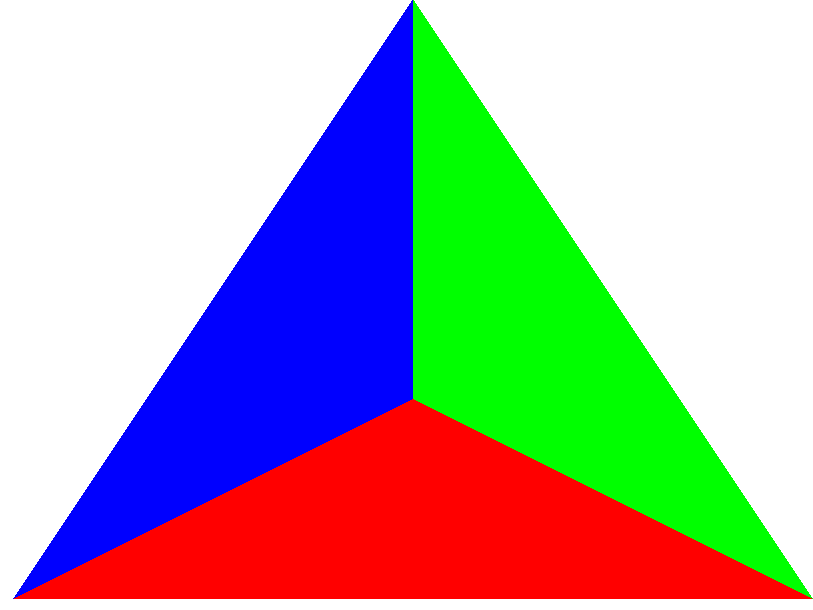
\includegraphics[scale=0.15]{images/min.png}
    \caption{Min diagram}\label{fig:min-diagram}
    \endminipage\hfill
    \minipage[b]{.5\linewidth}
    \centering
    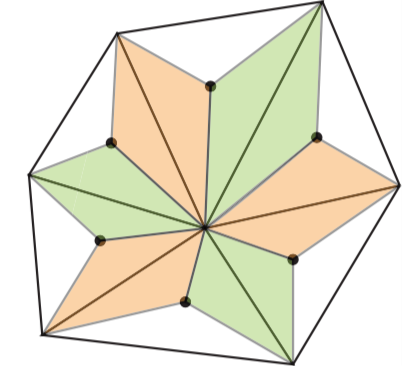
\includegraphics[scale=0.6]{images/edge-area.png}
    \caption{Region around an edge}\label{fig:edge-area}
    \endminipage
\end{figure}

\subsection{Min diagram - Edge based area} \label{section:max-diagram}
For each point in a triangle, we can easily determine its farthest vertex, which we use as a cue for coloring.
A different approach from interpolating, can be found coloring vertex areas based on the minimum barycentric coordinate.
The color is given by the region farthest from a vertex (Fig. \ref{fig:min-diagram}, Pseudocode \color{red}{insert Pseudocode}\color{black}).

\subsection{Mean Curvature}
TODO